
\documentclass[9pt,letterpaper,twoside]{article}


% Packages
\usepackage[spanish]{babel}
\usepackage{caption}
\usepackage[sfdefault,lf]{carlito}
\usepackage{datetime}
\usepackage{fancyhdr}
\usepackage{float}
\usepackage[T1]{fontenc}
\usepackage{geometry}
\usepackage{graphicx}
\usepackage[hidelinks]{hyperref}
\usepackage[utf8]{inputenc}
\usepackage{listings}
\usepackage{longtable}
\usepackage{multirow}
\usepackage{newfloat}
\usepackage{totcount}
\usepackage[table]{xcolor}
\usepackage{xurl}

% Macros
\newcommand{\printif}[3]{\ifcsname @#1\endcsname#2\else#3\fi}

% Variables
\makeatletter
  \def\institution#1{\gdef\@institution{#1}}
  \def\classcode#1{\gdef\@classcode{#1}}
  \def\classname#1{\gdef\@classname{#1}}
  \def\classsemester#1{\gdef\@classsemester{#1}}
  \def\classparallel#1{\gdef\@classparallel{#1}}
  \def\doctitle#1{\gdef\@doctitle{#1}}
  \def\docsubtitle#1{\gdef\@docsubtitle{#1}}
  \def\version#1{\gdef\@version{#1}}
  \def\astudentname#1{\gdef\@astudentname{#1}}
  \def\astudentlastname#1{\gdef\@astudentlastname{#1}}
  \def\astudentrol#1{\gdef\@astudentrol{#1}}
  \def\astudentemail#1{\gdef\@astudentemail{#1}}
  \def\bstudentname#1{\gdef\@bstudentname{#1}}
  \def\bstudentlastname#1{\gdef\@bstudentlastname{#1}}
  \def\bstudentrol#1{\gdef\@bstudentrol{#1}}
  \def\bstudentemail#1{\gdef\@bstudentemail{#1}}
  \def\cstudentname#1{\gdef\@cstudentname{#1}}
  \def\cstudentlastname#1{\gdef\@cstudentlastname{#1}}
  \def\cstudentrol#1{\gdef\@cstudentrol{#1}}
  \def\cstudentemail#1{\gdef\@cstudentemail{#1}}
\makeatother

% Page geometry
\geometry{
  letterpaper,
  top=1.0in,
  bottom=1.0in,
  left=1.25in,
  right=1.25in,
  headheight=15pt,
}
\setlength\parskip{1em}
\setlength\parindent{15pt}
\DeclareCaptionFormat{elements}{\captionsetup{justification=justified}\textbf{#1#2}#3\par}

% Header and footer
\pagestyle{fancy}
\cfoot{\thepage}
\renewcommand{\headrulewidth}{0.5pt}
\renewcommand{\footrulewidth}{0.5pt}
\makeatletter
  \fancyhead[LE]{\printif{classcode}{\@classcode\ - }{}\@classsemester}
  \fancyhead[RE]{\@doctitle}
  \fancyhead[LO]{\@astudentlastname\printif{bstudentlastname}{, \@bstudentlastname}{}\printif{cstudentlastname}{, \@cstudentlastname}{}}
  \fancyhead[RO]{\printif{version}{\@version\ - }{}\the\year/\two@digits{\month}/\two@digits{\day}}
\makeatother

% Tables configuration
\regtotcounter{table}

\captionsetup[table]{name=Tabla}
\captionsetup[table]{format=elements, singlelinecheck=false, margin=0pt, font={sf,footnotesize}}

% Figures configuration
\regtotcounter{figure}
\graphicspath{{figures/}}
\captionsetup[figure]{format=elements, singlelinecheck=false, margin=0pt, font={sf,footnotesize}}

% Code configurations
\DeclareFloatingEnvironment[fileext=loc]{code}
\regtotcounter{lstlisting}
\renewcommand\lstlistingname{Código}
\captionsetup[lstlisting]{format=elements, singlelinecheck=false, margin=0pt, font={sf,footnotesize}}
\lstset{
    inputencoding=utf8,
    extendedchars=true,
    literate=%
    {á}{{\'a}}1
    {é}{{\'e}}1
    {í}{{\'i}}1
    {ó}{{\'o}}1
    {ú}{{\'u}}1
    {Á}{{\'A}}1
    {É}{{\'E}}1
    {Í}{{\'I}}1
    {Ó}{{\'O}}1
    {Ú}{{\'U}}1
    {ñ}{{\~n}}1
    {Ñ}{{\~N}}1
}
\lstset{
    basicstyle=\small\ttfamily,
    backgroundcolor=\color{gray!10},
    keywordstyle=\color{blue},
    commentstyle=\color{green!40!black},
    stringstyle=\color{red},
    rulecolor=\color{gray},
    frame=single,
    framerule=0pt,
    framesep=2pt,
    captionpos=b,
    aboveskip=10pt,
    belowskip=5pt,
    columns=fullflexible,
    keepspaces=true,
    numberstyle=\tiny\color{gray},
    numbers=left,
    stepnumber=1,
    numbersep=5pt,
}
\lstdefinestyle{pythonstyle}{
    language=python
}
\lstnewenvironment{pythoncode}{\lstset{style=pythonstyle}}{}
\lstdefinestyle{bashstyle}{
    language=bash
}
\lstnewenvironment{bashcode}{\lstset{style=bashstyle}}{}
\lstdefinestyle{xmlstyle}{
    language=xml
}
\lstnewenvironment{xmlcode}{\lstset{style=xmlstyle}}{}
\lstdefinestyle{javastyle}{
    language=java
}
\lstnewenvironment{javacode}{\lstset{style=javastyle}}{}
\lstdefinestyle{plainstyle}{
}
\lstnewenvironment{plaincode}{\lstset{style=plainstyle}}{}

% Custom titlepage
\makeatletter
\def\@maketitle{
  % Configurations
  \renewcommand\listtablename{Índice de tablas}
  \renewcommand\lstlistlistingname{Índice de fragmentos de codigo}
  % Cover
  \thispagestyle{empty}
  \noindent\includegraphics[width=.475 \textwidth]{../latex-report-001/logo-\@institution}
  \vfill
  \vfill
  \begin{center}
    \printif{docsubtitle}{\fontsize{25}{25}\selectfont \@docsubtitle\\[3em]}{}
    {\fontsize{35}{35}\selectfont \@doctitle}\\[2.0em]
    {\fontsize{15}{15}\selectfont \printif{classcode}{\@classcode\ - }{}\@classsemester\printif{classparallel}{ - \@classparallel}{}}\\[10pt]
    {\fontsize{20}{20}\selectfont \@classname}\\[5pt]
    {\fontsize{15}{15}\selectfont \today\printif{version}{ - \@version}{}}
  \end{center}
  \vfill
  \vfill
  \vfill
  \begin{flushright}
    \begin{tabular}{r|l}
      \printif{astudentname}{\@astudentname\ \@astudentlastname & \@astudentrol \\ \@astudentemail & \\}{}
      \printif{bstudentname}{\@bstudentname\ \@bstudentlastname & \@bstudentrol \\ \@bstudentemail & \\}{}
      \printif{cstudentname}{\@cstudentname\ \@cstudentlastname & \@cstudentrol \\ \@cstudentemail & \\}{}
    \end{tabular}
  \end{flushright}
  \newpage
  % Index
  % Table of contents
  \tableofcontents
  % Tables
  \ifnum \totvalue{table}>0
    \listoftables
  \fi
  % Figures
  \ifnum \totvalue{figure}>0
    \listoffigures
  \fi
  % Code
  \ifnum \totvalue{lstlisting}>0
    \lstlistoflistings
  \fi
  \newpage
}
\makeatother

% Hooks
\AtBeginDocument{
  \maketitle
}


% Datos de la asignatura
\institution{utfsm}
\classcode{INF356}
\classname{Computación Distribuida para Big Data}
\classsemester{2025-1}
\classparallel{200}

% Datos de la entrega
\doctitle{Trabajo Práctico 1}
\version{v1.0}

% Estudiante
\astudentname{Miguel}
\astudentlastname{Soto}
\astudentrol{20430363-0}
\astudentemail{miguel.sotod@sansano.usm.cl}
  
\begin{document}

%%%%%%%%%%%%%%%%%%%%%%%%%%%%%%%%%%%%%%%%%%%%%%%%%%%%%%%%%%%%%%%%%%%%%%%%%%%%%%%%%%%
% Borrar o comentar esta sección instrucciones antes de entregar %%%%%%%%%%%%%%%%%%
%%%%%%%%%%%%%%%%%%%%%%%%%%%%%%%%%%%%%%%%%%%%%%%%%%%%%%%%%%%%%%%%%%%%%%%%%%%%%%%%%%%

\newpage

%%%%%%%%%%%%%%%%%%%%%%%%%%%%%%%%%%%%%%%%%%%%%%%%%%%%%%%%%%%%%%%%%%%%%%%%%%%%%%%%%%%
%%%%%%%%%%%%%%%%%%%%%%%%%%%%%%%%%%%%%%%%%%%%%%%%%%%%%%%%%%%%%%%%%%%%%%%%%%%%%%%%%%%
%%%%%%%%%%%%%%%%%%%%%%%%%%%%%%%%%%%%%%%%%%%%%%%%%%%%%%%%%%%%%%%%%%%%%%%%%%%%%%%%%%%

\section{Despligue del cluster}

\subsection{Implementación del tutorial}

\noindent
Para la creacion del Cluster en Amazon Web Services, fue necesario seguir los pasos indicados en el tutorial
entregado en el Slide T01 - Hadoop Cluster - v1.0 entregado en Aula. El instructivo constaba de los siguientes
pasos:
\begin{itemize}
    \item Crear la cuenta de AWS
    \item Preparar en entorno del Cluster
    \item Configurar la maquina Master
    \item Configurar todos los Workers
    \item Inicializar el Cluster
    \item Ejecutar el script de Map Reduce con Hadoop
\end{itemize}

\subsubsection*{Crear la cuenta de AWS}

\noindent
Para la creacion de la cuenta de AWS simplemente segui las indicaciones en el correo de invitacion indicado por el profesor.
Posterior a eso, me fui directamente a la seccion de Modules, en donde estaba el Modulo de Launch AWS Academy Learner Lab,
que sirve para entrar a la Console Home de AWS.

\subsubsection*{Preparar en entorno del Cluster}

\noindent
Una vez en Console Home, creamos una instancia de tipo EC2, para la cual creamos los Key Pairs, el Security Group y la instancia
Master.

\noindent
Para los Key Pairs, creamos una llave de tipo RSA con formato de archivo PEM.

\noindent
Para el Security Group, creamos tres reglas, 
una Inbound Rule de tipo SSH con tipo de fuente Anywhere-IPv4
para entrar por SSH,
una Inbound Rule de tipo Custom TCP con rango de puerto 8088 y tipo de fuente Anywhere-IPv4
para la consola web de Hadoop,
una Inbound Rule de tipo Custom TCP con rango de puerto 9870 y tipo de fuente Anywhere-IPv4
para la consola web de HDFS
y finalmente, una Inbound Rule de tipo Custom TCP con rango de puerto de 0 a 65535 y tipo de 
fuente Anywhere-IPv4.

\noindent
Para la instancia Master creamos un nodo con Ubuntu 24.04 de tipo t2.micro y con 16gb de almacenamiento.
Esta instancia usara la Key y Security Group recien creados (al igual que las instancias Worker mas adelante). 
Una vez configurados los parametros, lanzamos la instancia y nos conectamos por SSH:

\begin{code}[H]
    \lstinputlisting[style=bashstyle, caption={Conectarse por primera vez al Master usando la llave PEM con la IP publica}, label={code/ssh_into_master.sh}]{code/ssh_into_master.sh}
\end{code}

\subsubsection*{Configurar la maquina Master}

\noindent
El primer paso es logicamente actualizar los paquetes del sistema, para esto es necesario ejecutar el siguiente
comando:

\begin{code}[H]
    \lstinputlisting[style=bashstyle, caption={Actualizar repositorios locales y descargar actualizaciones}, label={code/update.sh}]{code/update.sh}
\end{code}

\noindent
Una vez hecho esto, instalamos el paquete correspondiente a Java / OpenJDK 11:

\begin{code}[H]
    \lstinputlisting[style=bashstyle, caption={Descargar Java / OpenJDK 11 usando APT}, label={code/install_java.sh}]{code/install_java.sh}
\end{code}

\noindent
Una vez que hayamos resuelto todos los paquetes necesarios, tenemos que crear una llave publica con el siguiente
comando:

\begin{code}[H]
    \lstinputlisting[style=bashstyle, caption={Crear una llave publica en formato RSA y autorizarla}, label={code/create_pub_key.sh}]{code/create_pub_key.sh}
\end{code}

\noindent
Esta llave publica la guardaremos en la carpeta de Authorized Keys para SSH, lo cual permitira al Master
conectarse a si mismo por LocalHost.

\noindent
Descargamos Hadoop 3.3.6 desde la pagina oficial usando el comando WGET, el cual hace una request a la pagina para descargar el archivo comprimido en formato
TAR GZ, el cual tendremos que descomprimir y modificar para indicarle parametros especiales. Ejecutamos entonces los siguientes comandos:

\begin{code}[H]
    \lstinputlisting[style=bashstyle, caption={Descargar y descomprimir Hadoop en el Master}, label={code/download_hadoop.sh}]{code/download_hadoop.sh}
\end{code}

\noindent
Esto creara una carpeta llamada hadoop-3.3.6 en el directorio Home del Master, esta carpeta albergara los binarios yu scripts ejecutables para desplegar nuestro Distributed File System (DFS).
Para poder ejecutar los comandos en dicha carpeta de manera directa, modificaremos las Variables de Entorno de la maquina Master, de esta manera podremos ejecutar los comandos en cualquier
directorio. Dichas Variables tambien contienen rutas para la ejecucion de OpenJDK y la ubicacion de nuestra carpeta Hadoop, las cuales debemos obedecer para que funcione correctamente nuestro
cluster. Las variables de entorno en Linux se guardan en el directorio /etc/environment y solo puede modificarse por el Super Usuario (Root). Personalmente, a mi me gusta usar Vim, pero para
aquellas personas con gustos inferiores existen alternativas:

\begin{code}[H]
    \lstinputlisting[style=bashstyle, caption={Editar las Variables de Entorno usando el usuario Root y el editor de texto Vim}, label={code/edit_env_vars.sh}]{code/edit_env_vars.sh}
\end{code}

\noindent
Las Variables debiesen quedar asi:

\begin{code}[H]
    \lstinputlisting[style=bashstyle, caption={Variables de Entorno que usaremos para el cluster}, label={code/env_vars.sh}]{code/env_vars.sh}
\end{code}

\newpage

\noindent
Lo ultimo es modificar los archivos de configuracion de Hadoop en base a lo indicado por el profesor. Estos archivos luego seran enviados a los Workers cuando comprimamos la carpeta hadoop-3.3.6.

\begin{code}[H]
    \lstinputlisting[style=bashstyle, caption={hadoop-3.3.6/etc/hadoop/core-site.xml}, label={code/core-site.xml}]{code/core-site.xml}
\end{code}

\begin{code}[H]
    \lstinputlisting[style=bashstyle, caption={hadoop-3.3.6/etc/hadoop/hdfs-site.xml}, label={code/hdfs-site.xml}]{code/hdfs-site.xml}
\end{code}

\newpage

\begin{code}[H]
    \lstinputlisting[style=bashstyle, caption={hadoop-3.3.6/etc/hadoop/mapred-site.xml}, label={code/mapred-site.xml}]{code/mapred-site.xml}
\end{code}

\begin{code}[H]
    \lstinputlisting[style=bashstyle, caption={hadoop-3.3.6/etc/hadoop/yarn-site.xml}, label={code/yarn-site.xml}]{code/yarn-site.xml}
\end{code}

\newpage

\subsubsection*{Configurar todos los Workers}

\noindent
Los Workers tambien seran maquinas con Ubuntu 24.04 y de tipo t2.micro, usaran las mismas Key Pairs y el mismo Security Group.
Lo unico que cambiara entre ellos y el Master sera el almacenamiento, las cuales constaran solo de 8gb en total.
Una vez creados los Workers desde el interfaz de EC2 de AWS, tendremos que obtener sus IP's publicas y privadas. La primera
para conectarnos por primera vez, la segunda para establecer una conexion permanente.
Anotamos las IP's privadas de la siguiente manera:

\begin{code}[H]
    \lstinputlisting[style=bashstyle, caption={IP's privadas de los Workers en la carpeta Home del Master}, label={code/worker_priv_ip.sh}]{code/worker_priv_ip.sh}
\end{code}

\noindent
Luego de tener esto, borramos el archivo comprimido de Hadoop que descargamos inicialmente y comprimimos el directorio que modificamos en el paso anterior para
luego enviarselo a los Workers. Estos luego descomprimiran el archivo de manera local para asi no abusar de nuestro ancho de banda limitado:

\begin{code}[H]
    \lstinputlisting[style=bashstyle, caption={Borrar el archivo hadoop-3.3.6.tar.gz y comprimimos el directorio hadoop-3.3.6}, label={code/arch_hadoop.sh}]{code/arch_hadoop.sh}
\end{code}

\noindent
Y como la tarea de configurar cada Worker manualmente es tedioso, usamos un script de Bash que realiza el trabajo por nosotros. El cual itera los siguientes pasos:

\noindent
Para cada una de las instancias Worker proceder de la siguiente forma:

\begin{enumerate}
\item Instalar la llave pública de la máquina Master en el Worker
\item Crear una llave para el Worker
\item Instalar la llave del Worker en el Master
\item Instalar la llave del Worker en el Worker
\item Actualizar el sistema operativo en el Worker
\item Instalar Java en el Worker (openjdk-11-jdk)
\item Editar el archivo /etc/environment de la misma forma que para Master
\item Reiniciar el worker
\item Transferir el archivo de despliegue de Hadoop de la máquina Master al Worker
\item Expandir el archivo de despliegue en la máquina Worker
\end{enumerate}

\noindent
El script utilizado quedo de la siguiente formula:

\begin{code}[H]
    \lstinputlisting[style=bashstyle, caption={Script para configurar todos los Workers desde el Master}, label={code/install1.sh}]{code/install1.sh}
\end{code}

\newpage

\begin{code}[H]
    \lstinputlisting[style=bashstyle, caption={Script para configurar todos los Workers desde el Master}, label={code/install2.sh}]{code/install2.sh}
\end{code}

Una vez configurado todo, reiniciamos el nodo Master y reingresamos cuando la maquina vuelva a estar activa.

\newpage

\subsubsection*{Inicializar el Cluster}

\noindent
Si las maquinas estan correctamente configuradas, podremos levantar el File System distribuido sin problemas.
Para esto es necesario formatear el disco e iniciar los servicios para la distribucion de este y para la gestion
de recursos entre los Workers. Cabe notar que por disco me refiero a unidad de almacenamiento, como vimos en
clases, un DFS no almacena datos de forma continua, si no que la reparte entre varios Nodos.

\noindent
Dicho esto, ejecutamos la siguiente serie de comandos:

\begin{code}[H]
    \lstinputlisting[style=bashstyle, caption={Formateamos el File System, lo iniciamos y llamamos al negociador de recursos YARN}, label={code/init_cluster.sh}]{code/init_cluster.sh}
\end{code}

\noindent
Luego, para corroborar de que todo esta en orden, ejecutamos el siguiente comando:

\begin{code}[H]
    \lstinputlisting[style=bashstyle, caption={Corroborar estado de nuestro HDFS}, label={code/hdfs-blocks1.sh}]{code/hdfs-blocks1.sh}
\end{code}

\noindent
La salida debiese ser algo del siguiente estilo:

\begin{code}[H]
    \lstinputlisting[style=bashstyle, caption={Estado del HDFS luego de haber ejecutado un Map Reduce}, label={code/hdfs-blocks2.sh}]{code/hdfs-blocks2.sh}
\end{code}

Notaremos que existe una seccion que muestra la cantidad de Data Nodes, si muestra 4 entonces configuramos correctamente
nuestro cluster.

\newpage

\subsubsection*{Ejecutar el script de Map Reduce con Hadoop}

Finalmente, ejecutamos nuestro algoritmo de Map Reduce. Para esto basta con crear un directorio /data, almacenar nuestro archivo
a leer y finalmente ejecutar el ejecutable JAR contenido en nuestra carpeta de Hadoop. Una vez hecho esto, podemos analizar la
salida del Map Reduce haciendole un Cat y pasandolo por Pipe a More para desplezgar la informacion por pantalla:

\begin{code}[H]
    \lstinputlisting[style=bashstyle, caption={Ejecutar el Map Reduce y leer su salida}, label={code/exec_map_reduce.sh}]{code/exec_map_reduce.sh}
\end{code}

\begin{figure}
    \centering
    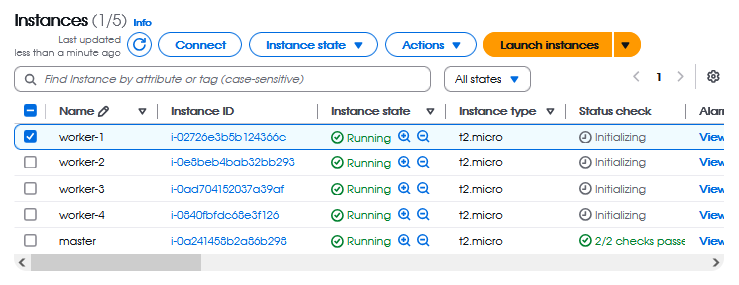
\includegraphics[width=\textwidth]{5-creacion_de_worker-3.PNG}
    \caption{Captura de pantalla de la ``AWS Management Console - EC2'' que muestra las máquinas del cluster creado con el tutorial}
    \label{5-creacion_de_worker-3.PNG}
\end{figure}

\newpage

\subsection{Expansión del cluster}

\noindent
Para expandir el cluster a 8 Workers, lo primero seria replicar las instancias desde AWS, estas debiesen tener los mismos
atributos que los workers originales. Lo segundo seria actualizar la configuracion desde el Master para incluir las nuevas
IP's y habilitar el uso de 4 Nodos desde los XML de Hadoop. Lo tercero seria configurar las conexiones de SSH hacia los workers
nuevos, para esto podemos reutilizar el script de Bash pero solo con las IP's privadas nuevas.

\begin{code}[H]
    \lstinputlisting[style=bashstyle, caption={Los archivos que hay que modificar antes de ejecutar el script de instalacion nuevamente}, label={code/expand_to_8.sh}]{code/expand_to_8.sh}
\end{code}

\newpage

\begin{figure}
    \centering
    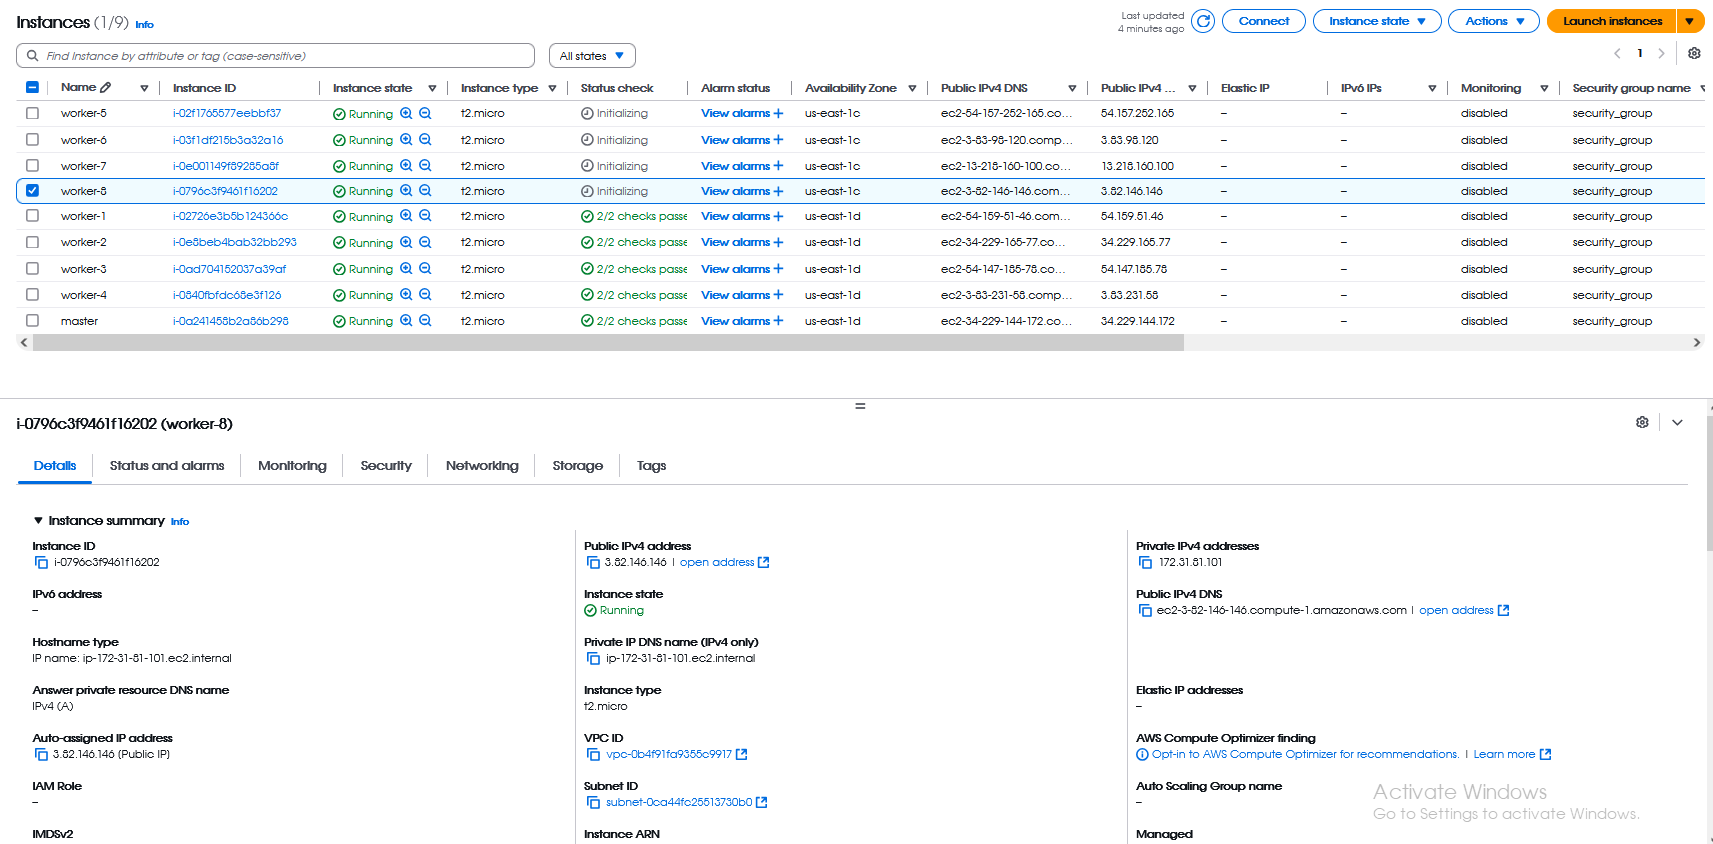
\includegraphics[width=\textwidth]{expanded_cluster_ec2}
    \caption{Captura de pantalla de la ``AWS Management Console - EC2'' que muestra las máquinas del cluster expandido}
    \label{expanded_cluster_ec2}
\end{figure}

\newpage

\subsection{Cliente web}

Aqui podemos apreciar todas las instancias desde la interfaz de EC2 de AWS, las instancias expandidas tienen el nombre de Worker
y un numoro que va desde 5 hasta 8. Sus direcciones IP privadas aparecen en el apartado de expansion y tienen las mismas
caracteristicas que los otros Nodos.

La figura \ref{hadoop.PNG} muestra la consola web de Hadoop y la figura \ref{hdfs.PNG} la consola web del HDFS.

\begin{figure}
    \centering
    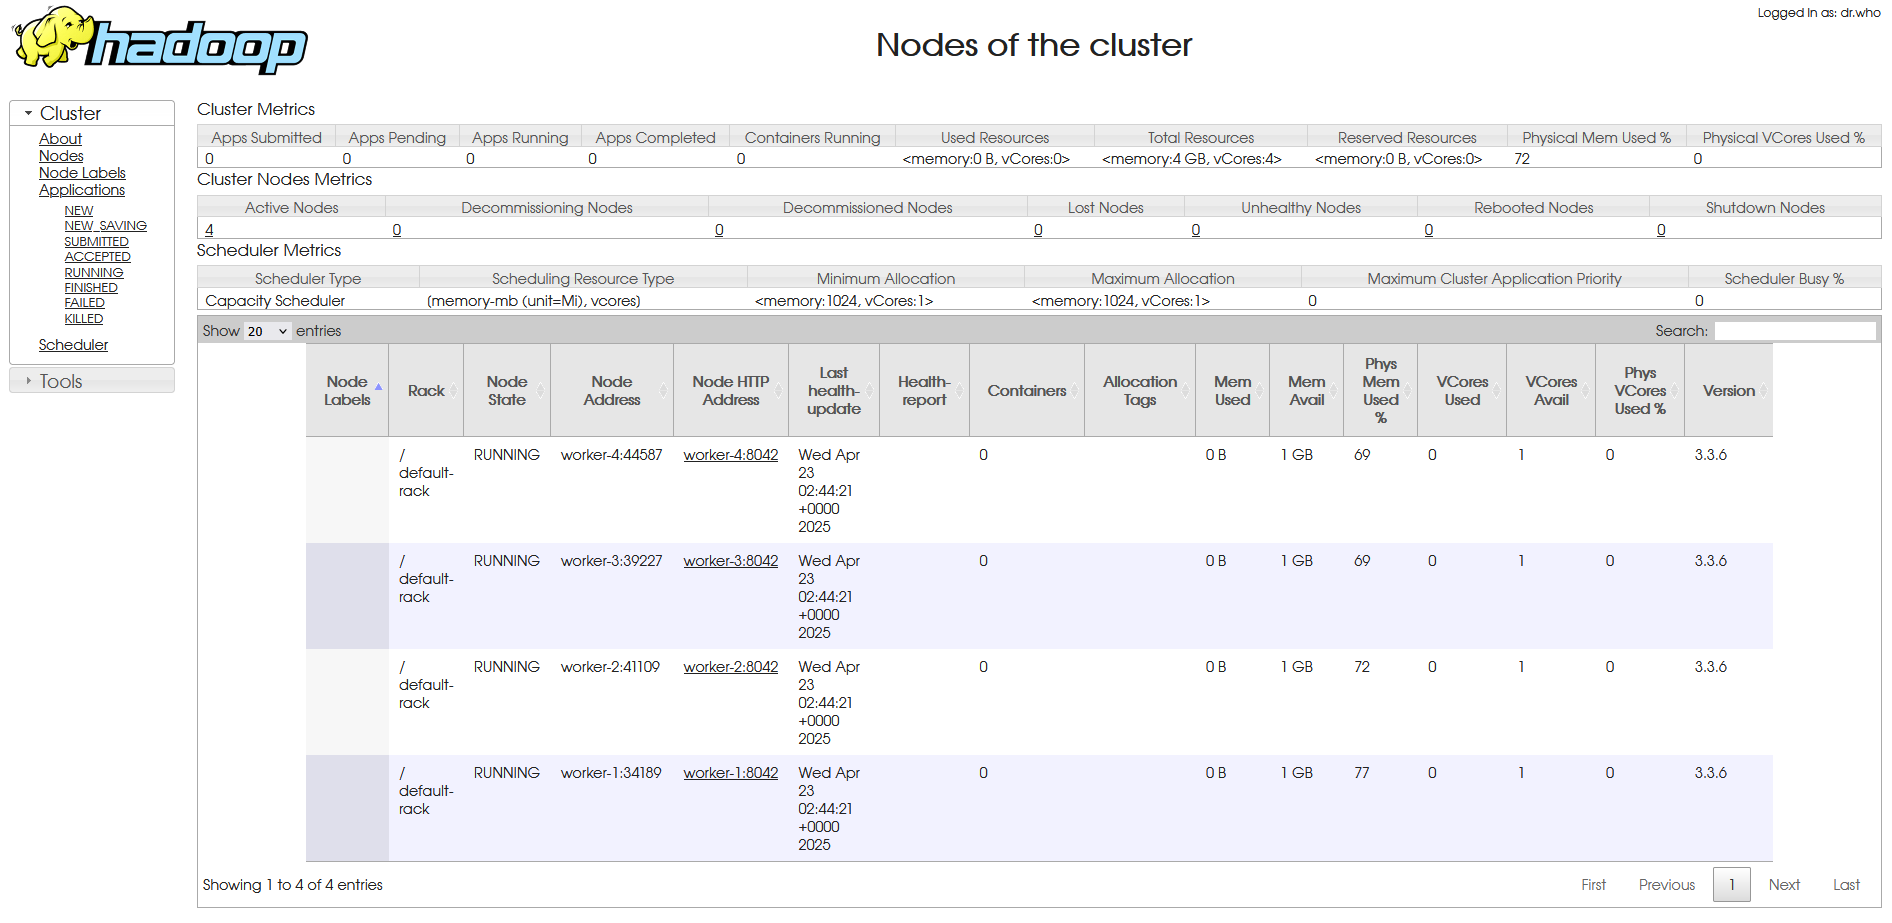
\includegraphics[width=\textwidth]{hadoop.PNG}
    \caption{Captura de pantalla del cliente web de Hadoop}
    \label{hadoop.PNG}
\end{figure}

\begin{figure}
    \centering
    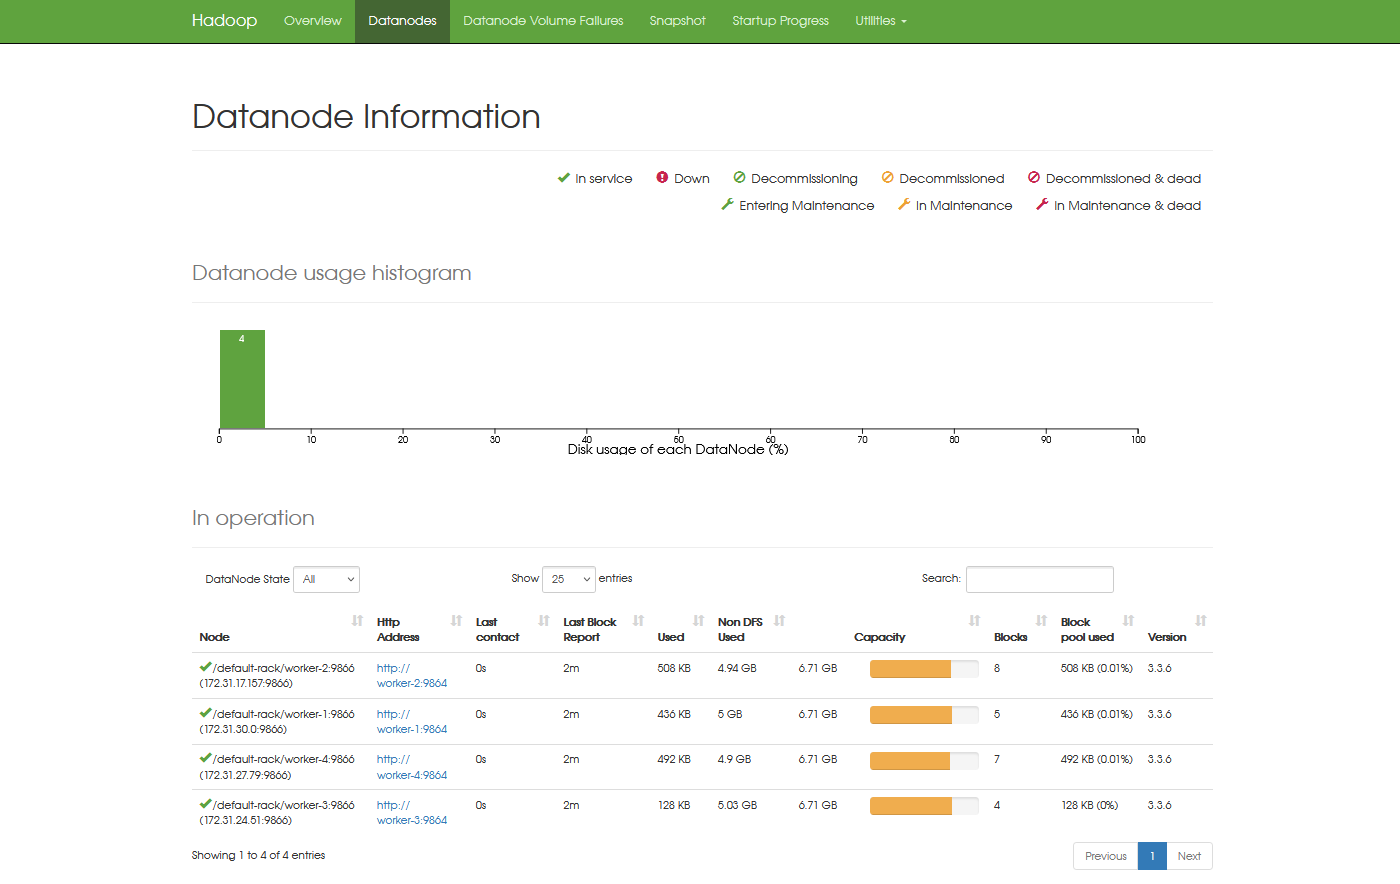
\includegraphics[width=\textwidth]{hdfs.PNG}
    \caption{Captura de pantalla del cliente web de HDFS}
    \label{hdfs.PNG}
\end{figure}

\newpage

\section{Instalación de Apache Hive}

\subsection{Procedimiento}

\noindent
Lo primero que debemos hacer para evitar cualquier posterior de cabeza grande, es ampliar
las capacidades de las instancias que tenemos construidas en AWS. Las mauinas Worker pasaran
a ser de tipo t3.small mientras que el Master a t3.medium. Esta mejora la realizamos desde
la interfaz de EC2 de AWS.

\begin{figure}
    \centering
    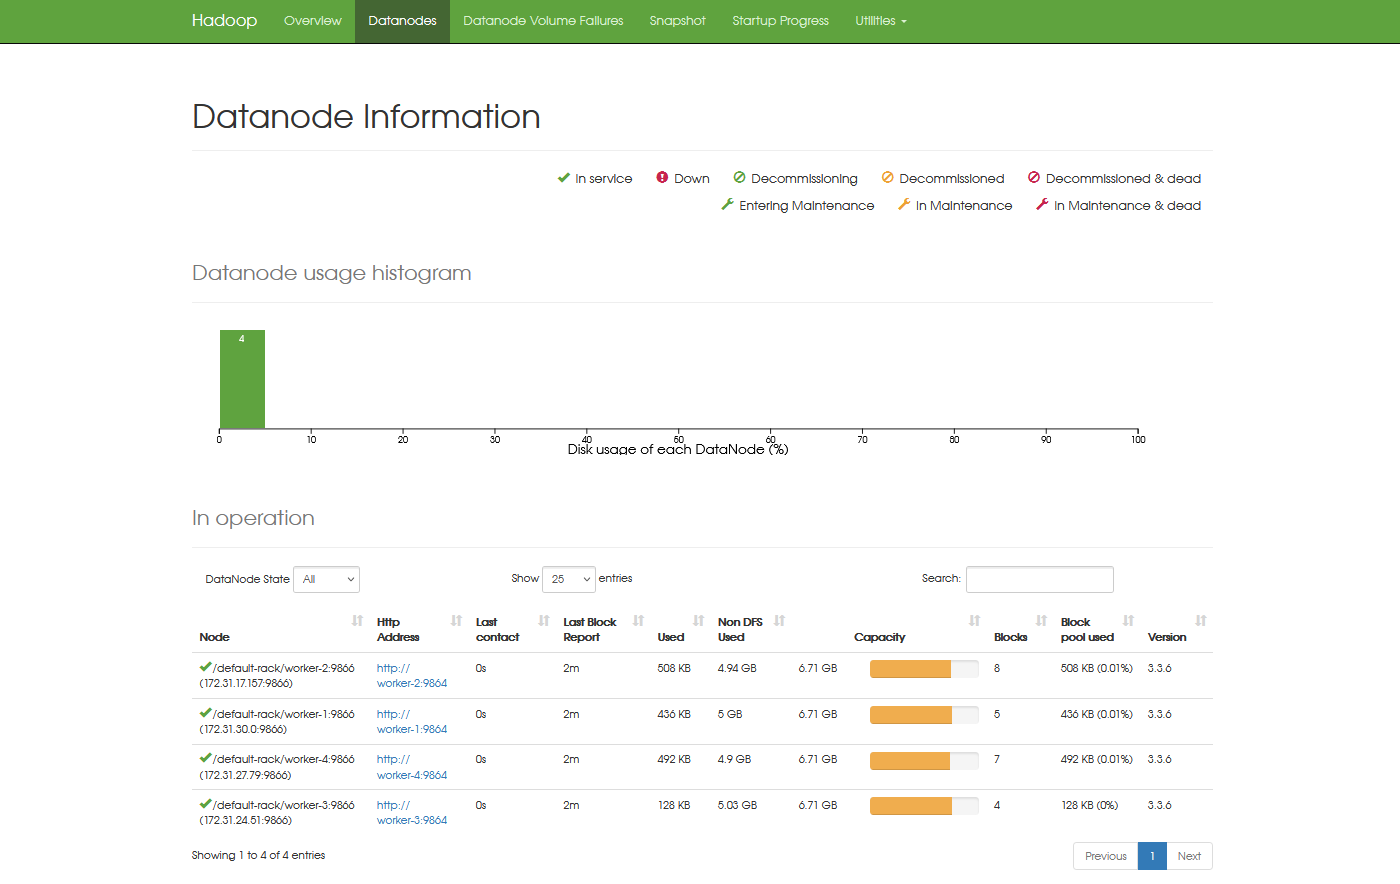
\includegraphics[width=\textwidth]{hdfs.PNG}
    \caption{Instancias mejoradas para no sufrir}
    \label{9-mejorar_los_nodos.png}
\end{figure}

\noindent
Lo segundo que hacemos es ir a la pagina oficial de Apache Hive para descargar la version
4.0.1. Desde el nodo Master tendremos que usar el comando WGET para descargar el comprimido correspondiente:

\begin{code}[H]
    \lstinputlisting[style=bashstyle, caption={Usar WGET para descargar Apache Hive 4.0.1}, label={code/down-hive.sh}]{code/down-hive.sh}
\end{code}

\noindent
Con el archivo ya descargado, lo descomprimimos de la misma manera que con Hadoop:

\begin{code}[H]
    \lstinputlisting[style=bashstyle, caption={Descomprimimos la carpeta de Apache Hive 4.0.1}, label={code/untar-hive.sh}]{code/untar-hive.sh}
\end{code}

\noindent
Luego, para poder utilizar el Apache Hive, debemos crear el archivo de configuracion necesario para que pueda funcionar por
sobre nuestra instalcion de Hadoop, para esto creamos el siguiente archivo XML y lo guardamos en 
/home/ubuntu/apache-hive-4.0.1-bin/conf/

\begin{code}[H]
    \lstinputlisting[style=bashstyle, caption={Archivo de configuracion de Apache Hive}, label={code/hive-site.xml}]{code/hive-site.xml}
\end{code}

\noindent
Creado dicho archivo, reiniciamos las maquinas.

\noindent
Con la maquinas ya reiniciadas, levantamos el servicio metastore y de hiveserver2 de la siguiente manera:

\begin{code}[H]
    \lstinputlisting[style=bashstyle, caption={Levantar MetaStore y HiveServer2}, label={code/metastore-n-hiveserver2.sh}]{code/metastore-n-hiveserver2.sh}
\end{code}

\noindent
Antes de seguir, es importante recordar que Apache Hive funciona por sobre Hadoop, por ende el DFS debe estar funcionando
al igual que el negociador de recursos, asi que los levantamos manualmente a traves de los scripts que vienen con Hadoop
de forma normal, luego, cuando ambos serivicios esten funcionando, corremos la shell de Apache Hive usando Beeline:

\begin{code}[H]
    \lstinputlisting[style=bashstyle, caption={Usar Beeline como interfaz a Hive}, label={code/beeline.sh}]{code/beeline.sh}
\end{code}

\newpage

\subsection{Prueba}

\noindent
Se nos entrega la Query a continuacion para probar el funcionamiento correcto de Hive:

\begin{code}[H]
\lstinputlisting[style=plainstyle, caption={Ejemplo de uso de Apache Hive}, label={lst:004}]{code/code-004.hql}
\end{code}

\noindent
Para corroborar que Hive funciona correctamente, descargue la salida completa tras ejecutar la Query anteriormente
mencionada. En las paginas siguientes esta la salida completa tras la ejecucion de dicho comando desde la Shell de
Beeline.

\newpage

\begin{code}[H]
    \lstinputlisting[style=plainstyle, caption={Salida de Apache Hive (Parte 1)}, label={code/hive-output-1.sh}]{code/hive-output-1.sh}
\end{code}

\newpage

\begin{code}[H]
    \lstinputlisting[style=plainstyle, caption={Salida de Apache Hive (Parte 2)}, label={code/hive-output-2.sh}]{code/hive-output-2.sh}
\end{code}

\newpage

\begin{code}[H]
    \lstinputlisting[style=plainstyle, caption={Salida de Apache Hive (Parte 3)}, label={code/hive-output-3.sh}]{code/hive-output-3.sh}
\end{code}

\newpage

\begin{code}[H]
    \lstinputlisting[style=plainstyle, caption={Salida de Apache Hive (Parte 4)}, label={code/hive-output-4.sh}]{code/hive-output-4.sh}
\end{code}

\newpage

\begin{code}[H]
    \lstinputlisting[style=plainstyle, caption={Salida de Apache Hive (Parte 5)}, label={code/hive-output-5.sh}]{code/hive-output-5.sh}
\end{code}

\newpage

\begin{code}[H]
    \lstinputlisting[style=plainstyle, caption={Salida de Apache Hive (Parte 6)}, label={code/hive-output-6.sh}]{code/hive-output-6.sh}
\end{code}

\begin{code}[H]
    \lstinputlisting[style=plainstyle, caption={Salida de Apache Hive (Parte 7)}, label={code/hive-output-7.sh}]{code/hive-output-7.sh}
\end{code}

\noindent
Mientras que la salida de referencia era:

\begin{code}[H]
\lstinputlisting[style=plainstyle, caption={Resultado esperado para ejemplo de uso de Apache Hive}, label={lst:005}]{code/code-005.txt}
\end{code}

\newpage

\section{Exploración del HDFS}

\noindent
Para desarrollar el Script que muestre algo similar a lo que sale a continuacion, me aproveche de la salida que tuve. En mi caso, se dio perfectamente
que Hadoop guardo el archivo en un unico bloque, por ende hice un Script en Bash que funcionara para mi
situacion especifica. De no ser asi el caso, hubiese guardado cada IP por bloque en archivos separados y luego
guardarlos en un arreglo usano un pipe desde LS.

\begin{code}[H]
\lstinputlisting[style=plainstyle, caption={Ejemplo de uso de Apache Hive}, label={lst:006}]{code/code-006.txt}
\end{code}

\noindent
El Script que hice fue el siguiente:

\begin{code}[H]
    \lstinputlisting[style=bashstyle, caption={Muestra el archivo, los bloques que ocupa, el factor de replicacion y la ubicacion de cada bloque}, label={code/hive-print-rep.sh}]{code/hive-print-rep.sh}
\end{code}

\newpage

\noindent
Para descargar el archivo solicitado, segui las intrucciones para instalar AWS CLI indicadas en la documentacion de AWS (https://docs.aws.amazon.com/cli/latest/userguide/getting-started-install.html)
y luego descargue el archivo usando el ultimo comando:

\begin{code}[H]
    \lstinputlisting[style=bashstyle, caption={Instalar AWS CLI}, label={code/aws-cli.sh}]{code/aws-cli.sh}
\end{code}

\newpage

\section{Uso del cluster}

\subsection{Importación}

\noindent
Primero, para determinar el orden correcto de los datos, los insertare de forma directa a la Base de Datos desde Hive, para esto hice una Query generada por un Script en donde
cada parametro recibe el nombre de parametro\_n, donde n es el numero de la columna, el cual se obtiene contando la cantidad de comas en la primera fila del archivo CSV. De 
forma preliminar todas las columnas seran de tipo String, ya que no tenemos forma de saber el tipo de dato de antemano.

\begin{code}[H]
    \lstinputlisting[style=bashstyle, caption={Importacion de los datos sucios}, label={importacion.sh}]{importacion.sh}
\end{code}

\newpage

\begin{code}[H]
    \lstinputlisting[style=bashstyle, caption={Importacion de los datos sucios}, label={importacion.hql}]{importacion.hql}
\end{code}

\noindent
Una vez con la Base de Datos generica creada, realizamos una Query para corroborar que los datos se insertaron correctamente.

\newpage

\subsection{Parsing}

\noindent
Al revizar los datos, notamos inmediatamente que el Script toma las comas que estan dentro de comillas dobles. Para solucionar esto cree un Script en Python que se encarga de borrar todas las
comas que se encuentran dentro de Strings con comillas dobles.

\begin{code}[H]
    \lstinputlisting[style=bashstyle, caption={Limpieza de los datos sucios}, label={cleanup.py}]{cleanup.py}
\end{code}

\noindent
Con los datos arreglados, realizamos otra tabla ya con los datos arreglados. Con esta tabla nueva creada, realizamos una Query para cada parametro en donde se devuelven los 100 valores unicos
por cada columna, de esta manera podemos saber que significa cada columna del CSV original para poder crear una ultima tabla con cada variable con un nombre y tipo mas apropiado.

\begin{code}[H]
    \lstinputlisting[style=bashstyle, caption={Importacion de los datos sucios}, label={importacion_limpia.hql}]{importacion_limpia.hql}
\end{code}

\newpage

\begin{code}[H]
    \lstinputlisting[style=bashstyle, caption={Analisis de los datos limpios para entender que significa cada columna}, label={output.hql}]{output.hql}
\end{code}

\noindent
Como ya hemos automatizado todo a este punto, le pasamos las tablas a nuestra LLM de preferencia y le preguntamos a que corresponden los datos devueltos por la Query.

\noindent

\newpage

\subsection{Análisis}

\noindent
En base a el analisis entregado por la Inteligencia Artificial, ademas de indagacion y criterio propio, la Query que agrupa los valores de cada columna con su nombre y tipo adecuado queda de la
siguiente forma:

\begin{code}[H]
    \lstinputlisting[style=bashstyle, caption={Observacion con nombres y tipos correctos}, label={obs_limpias_1.hql}]{obs_limpias_1.hql}
\end{code}

\newpage

\begin{code}[H]
    \lstinputlisting[style=bashstyle, caption={Observacion con nombres y tipos correctos}, label={obs_limpias_2.hql}]{obs_limpias_2.hql}
\end{code}

\end{document}
